\documentclass[letterpaper, 10pt]{report}
\title{Clemson Cyber Defense Hack Pack}
\author{Clemson ACM}
\date{\today}

\usepackage{makeidx}
\usepackage{multicol}
\usepackage{geometry}
\usepackage{tabularx}
\usepackage{pdfpages}
\geometry{margin=1in}

% Custom command for inline code.
\newcommand{\code}[1]{\texttt{#1}}

% Paragraph spacing should be easy!
\usepackage{parskip}

% Chapter title format: "X. Chaptertitle", not "Chapter X\nChaptertitle".
% Also, make \sections stand out a bit more.
\usepackage{titlesec}
\titleformat{\chapter}[block]{\normalfont\huge\bfseries}{\thechapter.}{1em}{\Huge}
\titleformat{\section}[block]{\normalfont\large\bfseries}{\thesection.}{1em}{\LARGE}

% Adjust spacing around headers to reduce empty space
\titlespacing*{\chapter}{0pt}{-22pt}{-1pt}
\titlespacing*{\section}{0pt}{10pt}{0pt}
\titlespacing*{\subsection}{0pt}{10pt}{0pt}
\titlespacing*{\subsubsection}{0pt}{0pt}{0pt}

% Citations should use superscript. It's nice.
\usepackage[superscript, biblabel]{cite}

% Use the Bera font family (based on Bitstream Vera) for text (bera), captions
% (berasans), and code (beramono).
\usepackage{bera}
\usepackage[scaled]{berasans}
\usepackage[scaled]{beramono}
\usepackage[T1]{fontenc}

% Needed for the inclusion of graphics.
\usepackage{graphicx}

% Allows the use of EPS files, a type of vector graphic.
\usepackage{epstopdf}

% Use the listings package for pretty source code inclusions.
\usepackage{color}
\usepackage{xcolor}
\usepackage{soul}
\usepackage{listings}
\lstset{
  basicstyle=\footnotesize\ttfamily, % Use a truetype, footnote-sized font.
  numbers=left,                      % line numbers go on the left
  numbersep=10pt,                    % how far the line-numbers are from the code
  tabsize=2,                         % sets default tabsize to 2 spaces
  extendedchars=true,                % lets you use non-ASCII characters; for 8-bits encodings only
  breaklines=true,                   % sets automatic line breaking
  keywordstyle=\bfseries,            % Keyword styling
  numberstyle=\ttfamily\color{gray}, % the style that is used for the line-numbers
  stringstyle=\color{gray},          % string literal style
  commentstyle=\itshape\color{gray}, % comment literal style
  title=\lstname,                    % show the filename of files included with \lstinputlisting
  frame=b,                           % show a frame along the bottom
  rulecolor=\color{lightgray},
  language=C++,                      % the default language of the code
  showspaces=false,                  % show spaces as space, not a litle underscore.
  showstringspaces=false             % same as above, in strings.
  showtabs=false,                    % same as above, with tabs.
  xleftmargin=17pt,
  framexleftmargin=17pt,
  framexrightmargin=5pt
}

% Listings caption configuration.
\usepackage{caption}
\DeclareCaptionFont{white}{\color{white}}
\DeclareCaptionFormat{listing}{\colorbox[cmyk]{0.43, 0.35, 0.35,0.01}{\parbox{\textwidth}{\vspace{1.5pt}\hspace{10pt}#1#2#3}}}
\captionsetup[lstlisting]{format=listing,labelfont=white,textfont=white, singlelinecheck=false, margin=0pt, font={bf, sf}}

% Defines a tikz frame for page-broken listing hints.
% Shamelessly stolen from https://tex.stackexchange.com/questions/77996/how-to-show-a-hint-when-lstlisting-is-breaking-page
\usepackage[framemethod=tikz]{./formatting/mdframed}
\mdfdefinestyle{note}
  {
    hidealllines = true ,
    skipabove    = .5\baselineskip ,
    skipbelow    = .5\baselineskip ,
    singleextra  = {} ,
    firstextra   = {
      \node[right,overlay,align=center,font=\continuingfont]
        at (O) {\continuingtext};
    } ,
    secondextra  = {
      \node[above right,overlay,align=left,font=\continuingfont]
        at (O |- P) {\continuedtext};
    } ,
    middleextra  = {
      \node[right,overlay,align=left,font=\continuingfont]
        at (O) {\continuingtext};
      \node[above right,overlay,align=left,font=\continuingfont]
        at (O |- P) {\continuedtext};
    }
  }

% Sets up the hint content and style for page-broken listings.
\newcommand*\continuingfont{\color{gray}\footnotesize\itshape}
\newcommand*\continuingtext{Continues on next page}
\newcommand*\continuedtext{Continued from previous page}

% A wrapper command for automatically wrapping input listings
% with a hintable frame.
\newcommand{\acmlisting}[2][]
{
\mdframed[style=note]
\lstinputlisting[#1]{#2}
\endmdframed
}

% Turn on the powerful indexing features
\makeindex

% Make links, footnotes, etc. clickable, and generate pdf bookmarks.
\usepackage{hyperref}
\hypersetup{
  pdfauthor={Clemson ACM, acm@cs.clemson.edu},
  pdfcreator={Clemson ACM, acm@cs.clemson.edu},
  pdftitle={Clemson ACM Hack Pack},
  pdfsubject={Clemson ACM Hack Pack},
  unicode=true,
  colorlinks=false,
  pdfborder=0 0 0,
  bookmarks=true
}



\begin{document}
\maketitle

#ifdef hackpackpp
\section*{Copyright}
Copyright (C) 2015 CLemson ACM \\
The contents of the .tex files are under a Creative Commons Attribution-ShareAlike 4.0
International License (CC-BY-SA 4.0). 
See https://creativecommons.org/licenses/by-sa/4.0/ for a copy of the license.

The content of all other files is available under the GPLv3 unless otherwise specified. \\
The Hackpack is a concise and extensive cheatsheet/guide designed to be used during cyber security competitions. \\
Copyright (C) 2015  Clemson ACM \\

This program is free software: you can redistribute it and/or modify
it under the terms of the GNU General Public License as published by
the Free Software Foundation, either version 3 of the License, or
(at your option) any later version.

This program is distributed in the hope that it will be useful,
but WITHOUT ANY WARRANTY; without even the implied warranty of
MERCHANTABILITY or FITNESS FOR A PARTICULAR PURPOSE\@.  See the
GNU General Public License for more details. \\

You should have received a copy of the GNU General Public License
along with this program.  If not, see <http://www.gnu.org/licenses/>.

\break
#endif



\begingroup
\let\clearpage\relax
\chapter*{10 Commandments of Cyber Defense}
\begin{multicols}{2}
\begin{enumerate}
    \item Thou shalt NEVER trust the red team
    \item Thou shalt trust but verify everything else
    \item Thou shalt know thy network
    \item Thou shalt patch your S!
    \item Thou shalt make frequent backups
    \item Thou shalt disable unused services
    \item Thou shalt set and use strong passwords
    \item Thou shalt always use a firewall
    \item Thou shalt log everything
    \item Thou shalt get your injects done on time
\end{enumerate}
\end{multicols}
\endgroup


\tableofcontents

\chapter{Essential Tools}

\chapter{Patching and Package Management}

\chapter{Users and Passwords}

\chapter{Auditing and Logs}

\chapter{Backups}

\chapter{Firewalls}

\index{firewall}
Firewalls are essentially sets of rules that allow network traffic in and out of a machine.
In general, firewalls should be configured to allow the minimum required access.
For Windows, the firewall is called Windows Firewall.
For Linux, iptables and firewalld are the most common firewalls.
For BSD, pf --- the basis of the pfsense enterprise firewall --- is the default.
Instructions for the Cisco ASA firewalls have also been included.

In general, there are 3 major elements of firewall security:

\begin{itemize}
	\item Use a default reject policy to avoid admitting unwanted traffic.
	\item Open only the required ports to make the services to work.
	\item Log any unusual traffic that hits the firewall.
\end{itemize}

\section{Iptables}\index{firewall!iptables}

Iptables stores the majority of its configuration in a series of files:
\begin{itemize}
	\item /etc/sysconfig/iptables --- where the iptables configuration stored in RedHat
		based distributions
	\item /etc/iptables --- where the iptables configuration is stored in Debian
		based distributions
	\item /etc/services --- an optional file that maps service names to port
		numbers
\end{itemize}

Iptables uses the following binaries:
\begin{itemize}
	\item iptables --- view and modify the firewall
	\item iptables-save --- prints the running configuration to stdout; Used to
		save the running configuration to a file.
	\item iptables-restore --- reads a file and sets the firewall configuration
\end{itemize}

While iptables does have a save file format, it is often configured via bash and the iptables command then saved and restored from the save file format after initial changes.
This is to avoid differences in the save file format between different version.
Iptables will stop processing a packet when it matches the first rule.
The only exception to this is the LOG target.
When the LOG target is matched, matching will continue; but the traffic will be
logged in the kernel log.

\acmlisting[caption=Iptables Script, label=Iptables Script]{./firewalls/configs/iptables.example}

\section{Firewalld}\index{firewall!firewalld}
firewalld references the following directories of files:

\begin{itemize}
	\item /usr/lib/firewalld --- where package default rules reside.
	\item /etc/firewalld --- where user overrides rules reside.
\end{itemize}

firewalld uses only the firewall-cmd binary.

firewalld is the new Linux firewall.
It provides a usability layer on top of iptables.
It focuses on zones and services.
Zones are affiliated with source address or interfaces.
Services define the ports that will be used with an application
It can be configured via scripts:

\acmlisting[caption=firewalld Script, label=firewalld Script]{./firewalls/configs/firewalld.example}

\section{pf}\index{firewall!pf}

pf references the following files:
\begin{itemize}
	\item /etc/rc.conf --- Like all bsd services, the pf service must be enabled here
	\item pf.conf  --- pf stores its configuration in the file.
\end{itemize}

Pf uses the following binaries
\begin{itemize}
	\item pfctl -f /etc/pf.conf --- load the firewall configuration
	\item pfctl -sa --- see the current configuration status
	\item kldload pf --- load the pf kernel module
\end{itemize}

All of the configuration for pf is stored in /etc/pf.conf.
There is no way to modify the running configuration except to overwrite the running
configuration with the saved configuration.
Unlike other firewalls, the last rule to match will be the rule that is applied.
This behavior can be overridden by using the `quick' keyword.

\acmlisting[caption=pf.conf, label=pf.conf]{./firewalls/configs/pf.conf.example}



\chapter{Services}

\chapter{Injects and Reports}

\bibliographystyle{plain}
\bibliography{hackpack}

\printindex

#ifdef hackpackpp
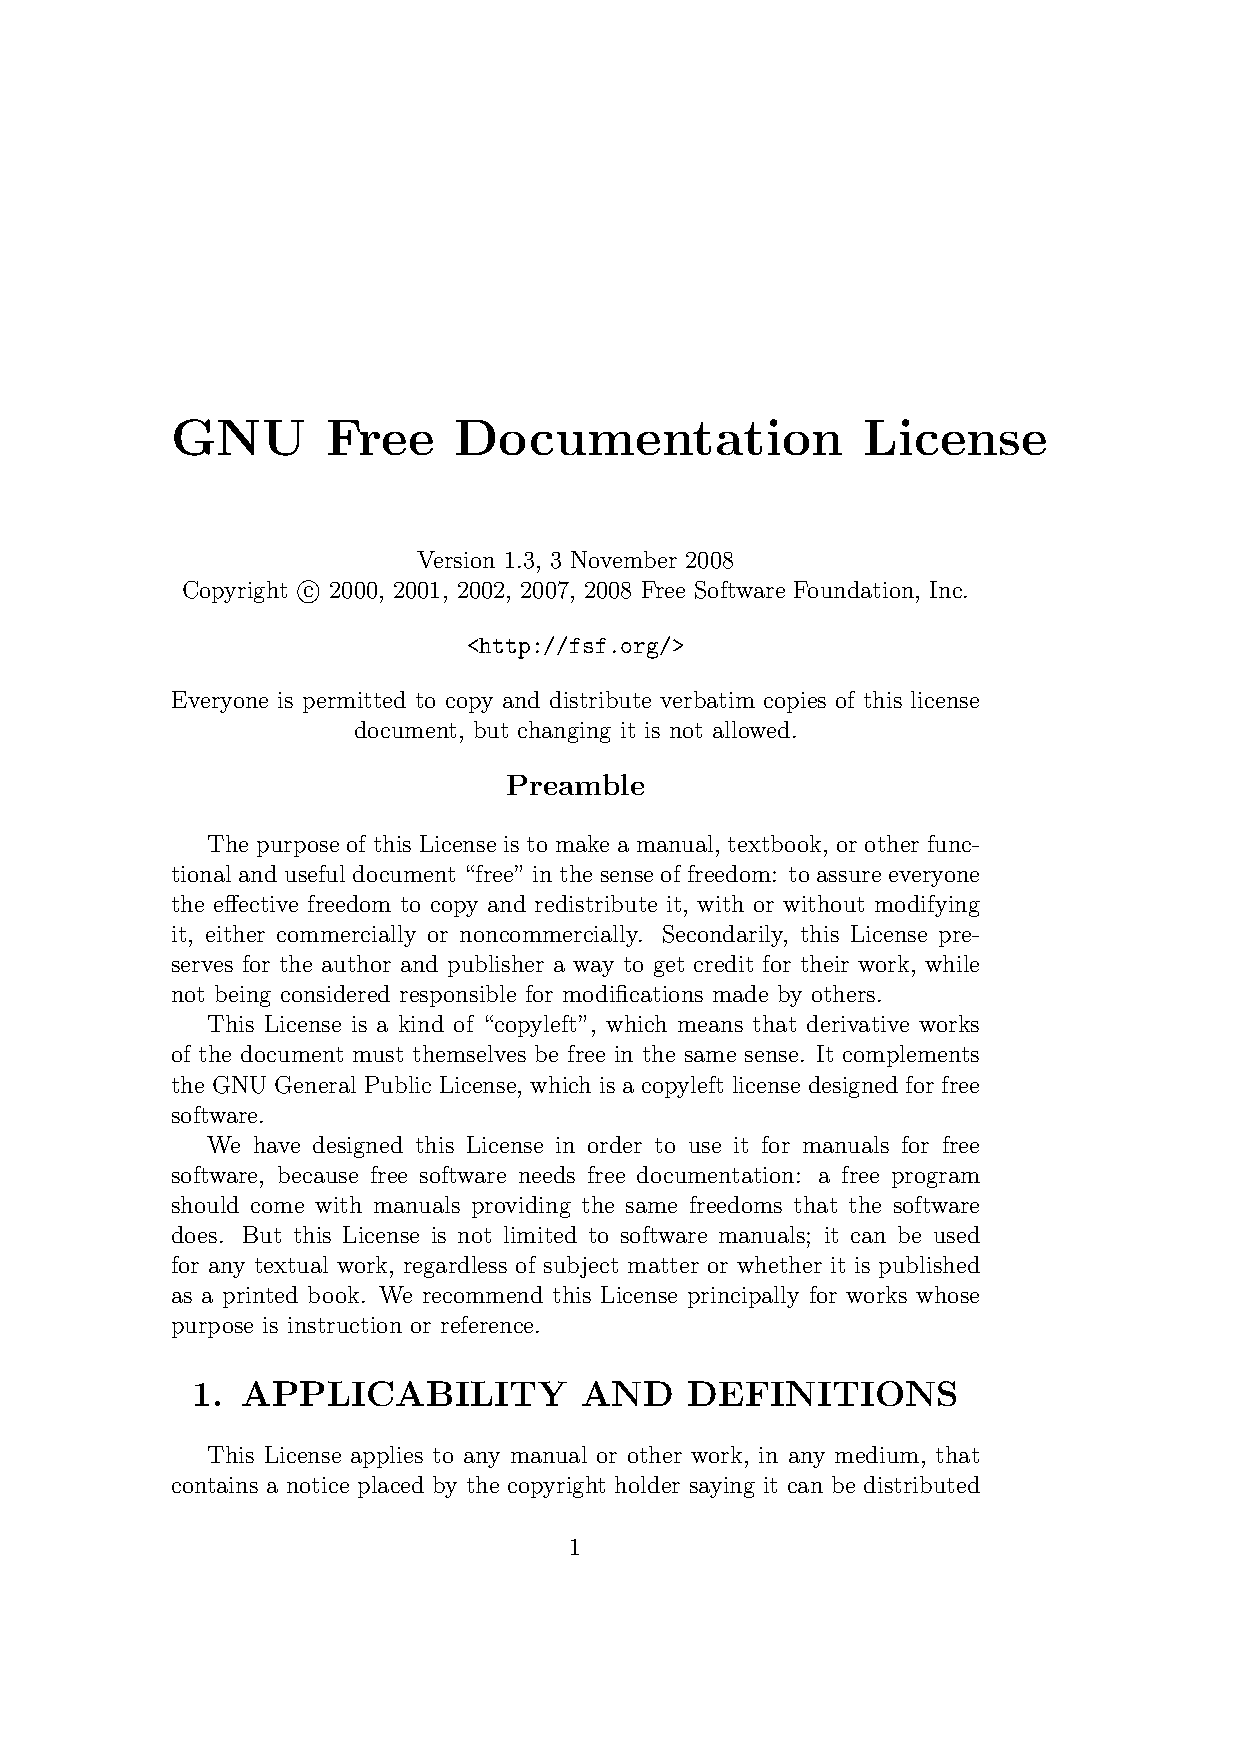
\includepdf[pages={-}]{./LICENCES/fdl.pdf}
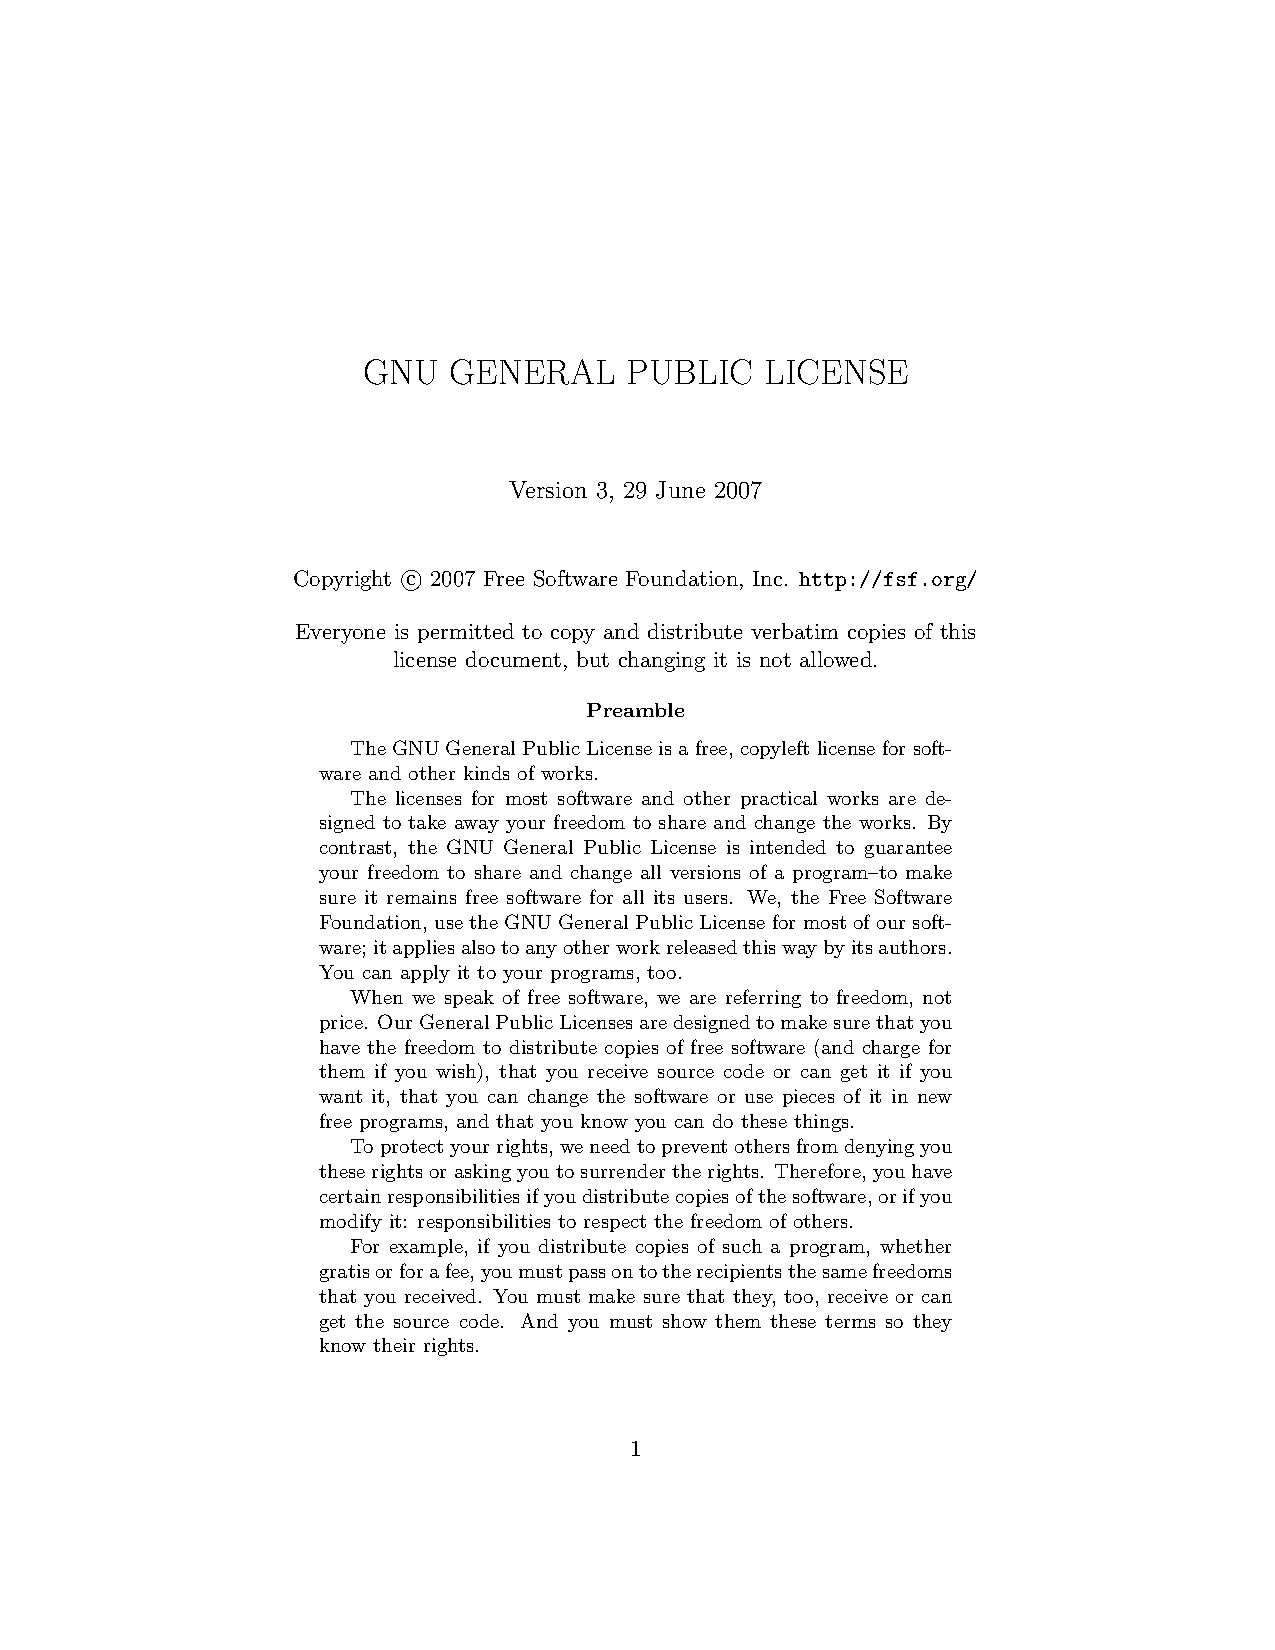
\includepdf[pages={-}]{./LICENCES/gpl.pdf}
#endif

\end{document}

